\documentclass[12pt]{article}
\usepackage[utf8]{inputenc}
\usepackage{amsmath}
\usepackage{systeme}
\usepackage{amsfonts}
\usepackage{graphicx}
\usepackage{enumitem}
\usepackage{hyperref}
\usepackage{xcolor}
\usepackage{kbordermatrix}
\usepackage{centernot}
\usepackage{xcolor}

\title{%
	\textbf{Notițe Seminar 6}}

\begin{document}
	
	\maketitle
	
	\textbf{{Intro:}} Până acum am făcut 2 algoritmi de clasificare: ID3, AdaBoost. Mai adăugam acum alți doi algoritmi: \textbf{Bayes Naiv} și \textbf{Bayes Corelat}.
	
	\textbf{Remember 1}
	
	Fie funcția $f : \{1,2,3\} \rightarrow \mathbb{R}$ cu $f(1) = 100, f(2) = 200, f(3) = 300$. Atunci:
	
	$$\max_{x \in \{1,2,3\}} f(x) = 300$$
	și 
	$$\arg \max_{x \in \{1,2,3\}} f(x) = 3$$
	
	
	
	
	\textbf{{Remember 2}}
	
	Ex.: Estimați în sensul verosimilății maxime (MLE) probabilitățile $P(A = 0,B = 0)$, $P(A=0|Y=1)$, având următorul tabel cu date:
	
	\begin{tabular}{ c | c || c }
		A & B & Y \\ 
		\hline
		0 & 0 & 0 \\  
		0 & 1 & 1 \\  
		1 & 0 & 1 \\  
		1 & 1 & 0
	\end{tabular}

	Vom nota cu $\#(\text{proprietăți})$ câte rânduri au anumite proprietăți. De exemplu: $\#(A=0)$  = (câte rânduri au $A=0$).

	$P(A=0,B=0) \stackrel{\text{MLE}}{=} \frac{\#(A=0,B=0)}{4} = \frac{1}{4}$
	
	$P(A=0|Y=1) \stackrel{\text{MLE}}{=} \frac{\#(A=0,Y=1)}{\#(Y=1)} = \frac{1}{2}$ (ne uităm doar la rândurile cu $Y=1$)
	
	\newpage
	\textbf{\large{Înspre clasificare bayesiană}}
	
	\begin{center}
		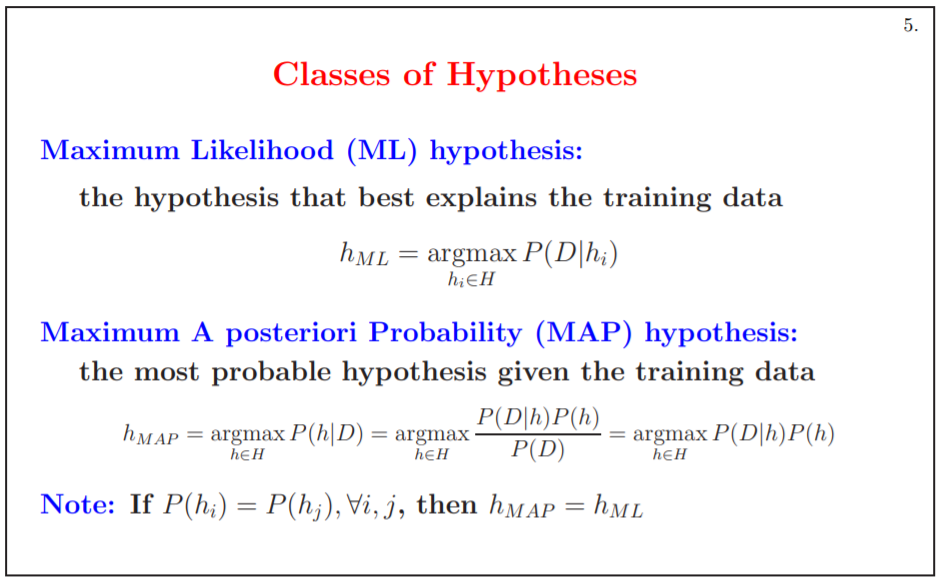
\includegraphics[width=1\linewidth]{screenshot001}
	\end{center}
	(slide preluat din \url{https://profs.info.uaic.ro/~ciortuz/SLIDES/ml6.pdf})
	
	Aplicare: Vezi ex. 3/pag. 370.
	
	\newpage
	
	\textbf{\large{Clasificare bayesiană}}
	
	\textbf{\large{Bayes Naiv}}
	\begin{center}
		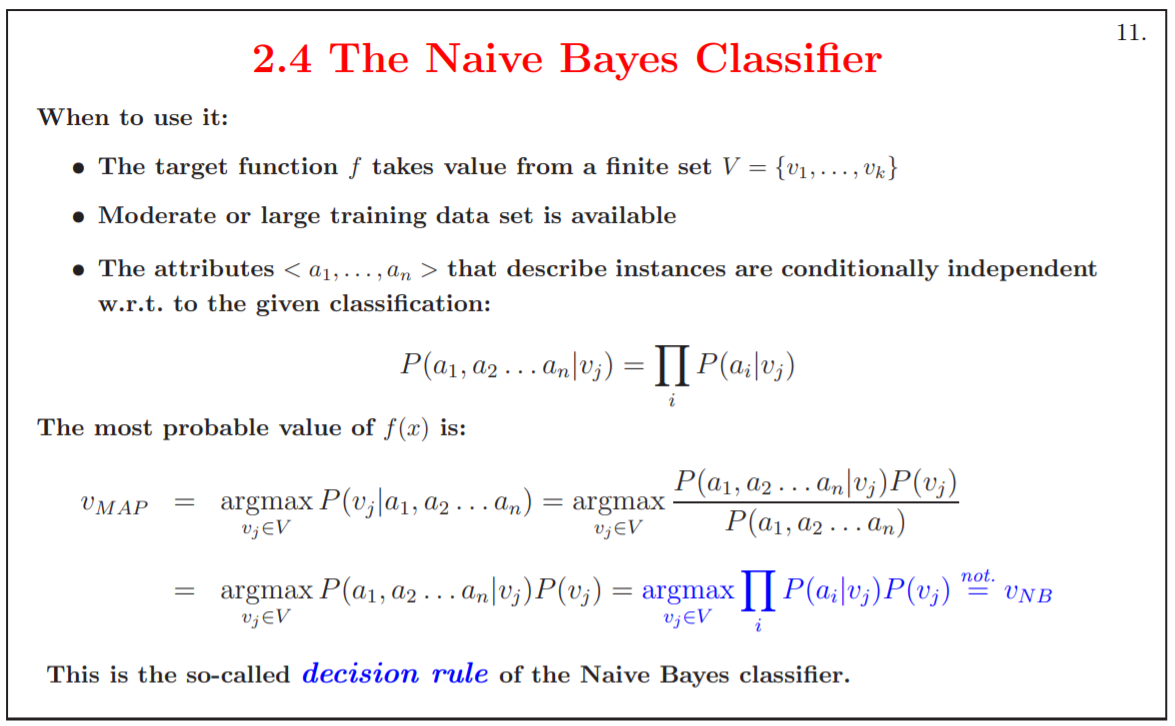
\includegraphics[width=1\linewidth]{screenshot002}
	\end{center}
	(slide preluat din \url{https://profs.info.uaic.ro/~ciortuz/SLIDES/ml6.pdf})
	
	Atribute de intrare: $A_1, \dots, A_n$
	
	Atributul de ieșire: $V$
	
	Antrenare: estimarea/calculul următoarelor probabilități:
	
	$P(v_j), \forall v_j \in \text{Val}(V)$
	
	$P(a_i | v_j), \forall a_i \in \text{Val}(A_i), \forall v_j \in \text{Val}(V)$
	
	Număr de parametri necesari de estimat: vezi ex. indicat mai jos
	
	Testare: utilizați regula de decizie din slide ($v_{NB}$).
	
	Algoritmul este \textit{naiv}, pentru că face presupunerea că atributele de intrare sunt independente condițional față de atributul de ieșire, lucru care nu se întâmplă de cele mai multe ori.
	
	\newpage
	
	\textbf{\large{Bayes Corelat}}
	\begin{center}
		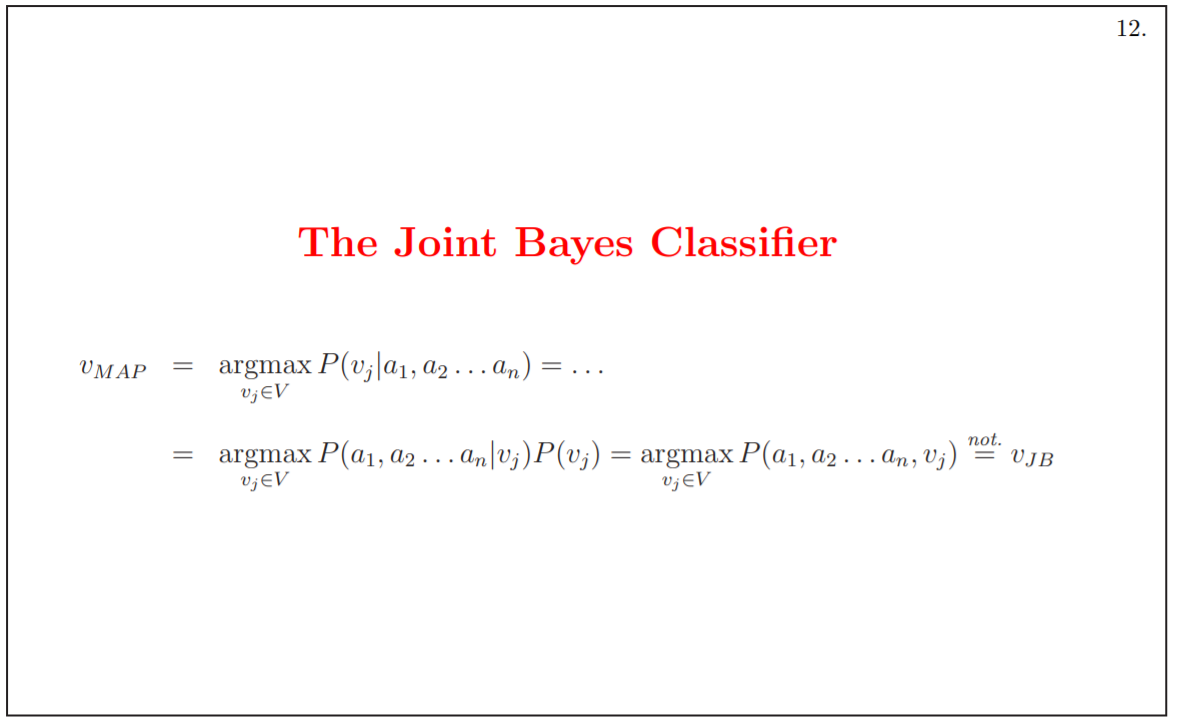
\includegraphics[width=1\linewidth]{screenshot003}
	\end{center}
	(slide preluat din \url{https://profs.info.uaic.ro/~ciortuz/SLIDES/ml6.pdf})
	
	Atribute de intrare: $A_1, \dots, A_n$
	
	Atributul de ieșire: $V$
	
	Antrenare: estimarea/calculul următoarelor probabilități:
	
	$P(v_j), \forall v_j \in \text{Val}(V)$

	$P(a_1,\dots,a_n|v_j), \forall a_i \in \text{Val}(A_i), \forall v_j \in \text{Val}(V)$

	Număr de parametri necesari de estimat: vezi ex. indicat mai jos

	Testare: utilizați regula de decizie din slide ($v_{JB}$).		
		\\
	Aplicare + altele (număr de parametri de estimat): vezi ex. 7/pag. 379	
	
	\newpage
	\textbf{{\large O altă perspectivă asupra algoritmilor Bayes naiv și Bayes corelat}}
	
	Regula de decizie a ambilor algoritmi poate fi scrisă și astfel:
	
	$\arg \max_{v_j \in \text{Val}(V)} P_{NB/JB}(a_1,\dots,a_n,v_j)$
	
	doar că unul calculează probabilitatea folosindu-se de distribuția presupusă de el (mă refer la Bayes naiv care presupune independența condițională a atributelor de intrare față de ieșire), iar altul calculează probabilitatea folosindu-se de distribuția reală.
	
	Altfel spus: având un rând la testare $(a_1,\dots,a_n)$, gândiți-vă la rândurile $(a_1,\dots,a_n,v_1)$, $(a_1,\dots,a_n,v_2)$, ..., $(a_1,\dots,a_n,v_k)$. Calculați probabilitatea fiecărui rând și returnați eticheta corespunzătoare probabilității maxime.
	
	\textbf{\large{Netezirea Laplace}}
	
	În cadrul algoritmului Bayes Naiv, când vreuna din probabilitățile $P(a_i|v_j)$ este 0, va fi o problemă pentru că produsul care apare în regula de decizie a lui Bayes Naiv va fi 0. Pentru a scăpa de acest neajuns, se folosește regula lui Laplace (netezirea de tip \textit{add-one}):
	
	$$P(A_i=a_i|V=v_j) \stackrel{\text{Laplace}}{=} \frac{\#(A_i=a_i,V=v_j) + 1}{\#(V=v_j) + |\text{Val}(A_i)|}$$
	
	Vă amintesc că fără regula lui Laplace era astfel:
	
	$$P(A_i=a_i|V=v_j) \stackrel{\text{MLE}}{=} \frac{\#(A_i=a_i,V=v_j)}{\#(V=v_j)}$$
	
	Aplicare: vezi ex. 6/pag. 377
	
	Dacă vreți să înțelegeți de unde vine formula, citiți în continuare:
	
	Suntem în contextul ex. 6b/pag. 377 și vrem să calculăm $P(\text{study}=1|\text{category = spam})$, $P(\text{study}=1|\text{category = regular})$ cu regula lui Laplace.
	
	Vom construi un tabel cu frecvențe (valoarea din prima celulă va fi egală cu numărul de rânduri cu study = 0 și category = regular):
	
	 \begin{tabular}{ c | c | c }
	 	 & category = regular & category = spam \\ 
	 	\hline
	 	study = 0 & 1 & 8 \\  
	 	study = 1 & 3 & 0 \\
	 	\hline \hline
	 	& 4 & 8
	 \end{tabular}
	
	Astfel, am putea scrie:
	
	$$P(\text{study}=1|\text{category = regular}) \stackrel{\text{MLE}}{=} \frac{3}{4}$$
	
	$$P(\text{study}=1|\text{category = spam}) \stackrel{\text{MLE}}{=} \frac{0}{8}$$
	
	Pentru că avem o celulă cu zero, atunci refacem tabelul adăugând 1 (\textit{add-one}...) la fiecare celulă:
	
	\begin{tabular}{ c | c | c }
		& category = regular & category = spam \\ 
		\hline
		study = 0 & 2 & 9 \\  
		study = 1 & 4 & 1 \\
		\hline \hline
		& 6 & 10
	\end{tabular}

	Astfel, putem scrie:
	
	$$P(\text{study}=1|\text{category = regular}) \stackrel{\text{Laplace}}{=} \frac{4}{6}$$
	
	$$P(\text{study}=1|\text{category = spam}) \stackrel{\text{Laplace}}{=} \frac{1}{10}$$
	
	\newpage
	\textbf{\large{Schemă de final}}
	\begin{enumerate}
		\item Ipoteze \begin{enumerate}
			\item ML
			\item MAP
		\end{enumerate}
		\item Bayes Naiv
		\begin{enumerate}
			\item Antrenare
			\begin{enumerate}
				\item algoritm
				\item număr de parametri de estimat 
			\end{enumerate}
			\item Testare
		\end{enumerate}
		\item Bayes Corelat
		\begin{enumerate}
			\item Antrenare
			\begin{enumerate}
				\item algoritm
				\item număr de parametri de estimat 
			\end{enumerate}
			\item Testare
		\end{enumerate}
		\item O altă perspectivă asupra alg. BN, JB
		\item Netezirea Laplace
		
	\end{enumerate}
	
\end{document}